\subsection{Schematischer Aufbau der Wärmepumpe}
Eine Wärmepumpe ist typischerweise wie in Abbildung \ref{fig:1} aufgebaut.
\begin{figure}
\centering
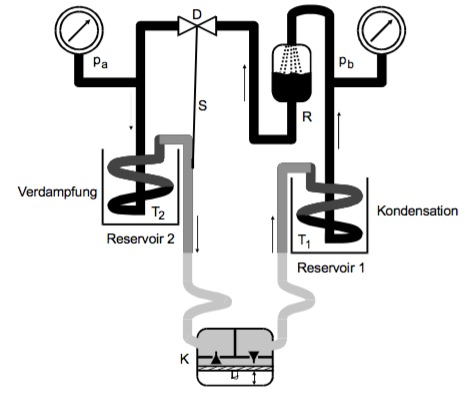
\includegraphics[width=10cm]{Bilder/schema.jpg}
\caption{schematischer Aufbau einer Wärmepumpe\,\cite{206}}
\label{fig:1}
\end{figure}
In der Wärmepumpe befindet sich ein reales Gas, welches durch Verdampfung Wärme aufnimmt
und sie bei Kondesation wieder abgibt. Dies wird als Phasenumwandlungsenergie bezeichnet
und es sollte idealerweise ein Gas mit hoher Kondensationswärme verwendet werden, damit
der Wirkungsgrad möglichst groß ist.

Das Gas bewegt sich im Kreislauf, welcher durch den Kompressor $K$ erzeugt wird. Dabei
durchströmt das Gas zwei Reservoire und das dazwischen liegende Drosselventil $D$.
An diesem Ventil entsteht ein Druckunterschied $p_\su{b}-p_\su{a}$. Dieses Ventil wird
über die Temperaturdifferenz gesteuert, da nur Gase in den Kompressor gelangen dürfen.

Im ersten Reservoir ist das Gas mit der Temperatur $T_\su{1}$ und dem Druck $p_\su{b}$
flüssig, im zweiten Reservoir ist das Gas mit der Temperatur $T_\su{2}$ und dem Druck
$p_\su{a}$ gasförmig. Das Wasser verdampft dann beim Durchströmen des Drosselventils
im zweiten Reservoir und entzieht diesem somit die Verdampfungswärme $L$. Das kalte, zweite
Reservoir, gibt somit Wärme ab.
Danach wird das Gas im Kompressor adiabatisch komprimiert, wodurch der Druck und die Temperatur
soweit ansteigen, bis sich das Gas im ersten Reservoir wieder verflüssigt. Hier wird die
Verdampfungswärme wieder abgegeben. Dadurch wird das erste Reservoir wieder aufgeheizt.
\subsection{Durchführung}
Für den vorliegenden Versuch wird der Aufbau aus Abbildung \ref{fig:2} verwendet.
\begin{figure}
  \centering
  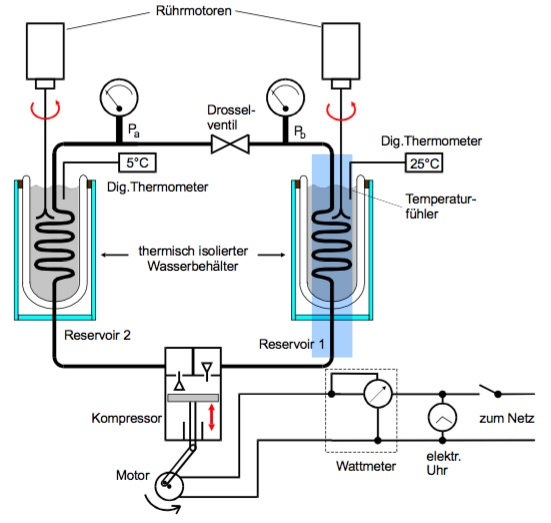
\includegraphics[width=0.7\textwidth]{Bilder/aufbau.jpg}
  \caption{Aufbau der Messaparatur \,\cite{206}}
  \label{fig:2}
\end{figure}
Dabei werden die beiden Reservoire jeweils mit $3 \,\si{\liter}$ Wasser befüllt. Danach
werden die Rührmotoren angestellt, bevor die Messung startet. Dann wird der Kompressor
angeschaltet. Von hier an werden die Drücke $p_\su{a}$, $p_\su{b}$, die Temperaturen
$T_\su{1}$, $T_\su{2}$ und die Leistung $N_\su{mech}$ im Abstand von $1\,\si{\minute}$
abgelesen und notiert. Die Messung endet, wenn $T_\su{1} = 50\,\si{\celsius}$ erreicht wird.
